\documentclass[aps,prd,twocolumn,showpacs,superscriptaddress,groupedaddress,nofootinbib]{revtex4}  % for review and submission
%\documentclass[aps,preprint,showpacs,superscriptaddress,groupedaddress]{revtex4}  % for double-spaced preprint
\usepackage{graphicx}  % needed for figures
\usepackage{dcolumn}   % needed for some tables
\usepackage{bm}        % for math
\usepackage{amsmath,amssymb}   % for math
\usepackage{aas_macros}
\usepackage{multirow}
\usepackage{color}
\usepackage{verbatim}
%\usepackage{times}
\usepackage{url}
\usepackage{hyperref}

% avoids incorrect hyphenation, added Nov/08 by SSR
\hyphenation{ALPGEN}
\hyphenation{EVTGEN}
\hyphenation{PYTHIA}

\newcommand{\mr}{\mathrm}
\newcommand{\tcb}{\textcolor{blue}}
\newcommand{\bea}{\begin{eqnarray}}
\newcommand{\eea}{\end{eqnarray}}
\newcommand{\bmp}{\bm{\Psi}}
\newcommand{\bms}{\bm{s}}
\newcommand{\bmk}{\bm{k}}
\newcommand{\bmx}{\bm{x}}
\newcommand{\bmq}{\bm{q}}
\newcommand{\la}{\langle}
\newcommand{\ra}{\rangle}

\begin{document}
% The following information is for internal review, please remove them for submission
\widetext
% the following line is for submission, including submission to the arXiv!!
%\hspace{5.2in} \mbox{Fermilab-Pub-04/xxx-E}

\title{Nonlinear Reconstruction}
%\title{Reconstruction beyond the Zel'dovich approximation}
%\title{Moving mesh reconstruction} 

\author{New paradigm}
\affiliation{in the Large-scale structure}

%\author{Hong-Ming Zhu}
%\affiliation{Key Laboratory for Computational Astrophysics, National Astronomical Observatories, Chinese Academy of Sciences, 20A Datun Road, Beijing 100012, China}
%\affiliation{University of Chinese Academy of Sciences, Beijing 100049, China}

%\author{Yu Yu}
%\affiliation{Key Laboratory for Research in Galaxies and Cosmology,
%Shanghai Astronomical Observatory, Chinese Academy of Sciences,
%80 Nandan Road, Shanghai 200030, China}

%\author{Ue-Li Pen}
%\affiliation{Canadian Institute for Theoretical Astrophysics, University of Toronto, 60 St. George Street, Toronto, Ontario M5S 3H8, Canada}
%\affiliation{Dunlap Institute for Astronomy and Astrophysics, University of Toronto, 50 St. George Street, Toronto, Ontario M5S 3H4, Canada}
%\affiliation{Canadian Institute for Advanced Research, CIFAR Program in Gravitation and Cosmology, Toronto, Ontario M5G 1Z8, Canada}
%\affiliation{Perimeter Institute for Theoretical Physics, 31 Caroline Street North, Waterloo, Ontario, N2L 2Y5, Canada}

%\author{Matthew McQuinn}
%\affiliation{Department of Astronomy, University of Washington, Seattle, WA 98195, USA}

%\author{Xuelei Chen}
%\affiliation{Key Laboratory for Computational Astrophysics, National Astronomical Observatories, Chinese Academy of Sciences, 20A Datun Road, Beijing 100012, China}
%\affiliation{University of Chinese Academy of Sciences, Beijing 100049, China}
%\affiliation{Center of High Energy Physics, Peking University, Beijing 100871, China}

\date{\today}

\begin{abstract}
We present a new method to reconstruct the primordial (linear) density field
using the estimated nonlinear displacement field. The divergence of 
the displacement field gives the reconstructed density field. We solve the 
nonlinear displacement field ... ... 
\end{abstract}

\pacs{}
\maketitle

%\section{\label{sec:level1}First-level heading}
% sections are not used for PRL papers

{\it Introduction.}---The observed large-scale structure provides ...
In this Letter, we solve the nonlinear displecement field from the nonlinear 
density field and present a new method to reconstruct the primordial density
field and hence the linear BAO information.

The analysis usually uses the density field directly. measure the power spectrum
However, modeling the small-scale inhomogeneities limits to $k<0.1\ h/\mr{Mpc}$.
We find the nonlinearities in the displacement field is much more linear than 
the density field. The correlation of the divergence of the displacement field
with the primordial (linear) density field is much better than that of the 
nonlinear density field. The divergence of the reconstructed nonlinear
displacement gives the reconstructed density field, which is much more linear
than the nonlinear density field.

%=========

{\it Displacement decomposition.}---In the Lagrangian picture of structure 
formation, 
the displacement field $\bm{s}(\bm{q},\tau)$ fully describes the motion of each mass element. The Eulerian position $\bm{x}$ of a mass element is given by
\bea
\bm{x}(\bm{q},\tau)=\bm{q}+\bm{s}(\bm{q},\tau),
\eea
where $\bm{q}$ is the initial Lagrangian position of this mass element.
The displacement field $\bm{s}(\bm{q})$ can be decomposed into a gradient part
and a curl part,
\bea
\bm{s}(\bm{q})=\bm{s}_E(\bm{q})+\bm{s}_B(\bm{q}),
\eea
where $\nabla\times\bm{s}_E=0$ and $\nabla\cdot\bm{s}_B=0$.
The gradient part can be completely described by a scalar potential,
while the curl part has two independent components.

In the 1D cosmology, the displacement field has only one component though 
it is a vector field \cite{2016matt}. 
This allows us to determine the displacement field, which is a vector field, 
from the density field, which is a scalar field \cite{2016arXiv160907041Z}.
However, the motion has three degrees of freedom in 3D instead of one.
Since from cosmological observations we only have the density field, we expect 
to reconstruct the scalar part of the displacement field.

%=========

{\it Reconstruction algorithm.}---The basic idea is to build a curvilinear 
coordinate system $\bm{\xi}\equiv(\xi_1,\ \xi_2,\ \xi_3)$, where the mass per
volume element is constant \cite{1995ApJS..100..269P,1998ApJS..115...19P}. 
In order to determine the physical position of each grid point, we need to 
specify the Cartesian coordinate $\bm{x}(\bm{\xi},\ t)$ of each curvilinear 
coordinate.
As in Refs.\cite{1995ApJS..100..269P,1998ApJS..115...19P}, we define a coordinate transformation that is a pure gradient,
\bea
x^i=\xi^\mu\delta^i_\mu+\Delta x^i,
\eea
where
\bea
\Delta x^i\equiv\frac{\partial\phi}{\partial\xi^\nu}\delta^{i\nu}.
\eea
Here, $\Delta\bm{x}$ is called the {\it lattice displacement} and $\phi$ the 
{\it deformation potential} \cite{1995ApJS..100..269P,1998ApJS..115...19P}.
Here, Latin indices denote Cartesian coordinate labels $x^i$, Greek indices 
imply curvilinear coordinates $\xi^\alpha$.

One efficient algorithm to solve the deformation potential is the moving mesh
method \cite{1995ApJS..100..269P,1998ApJS..115...19P}.
The moving mesh method is originally introduced for 
\bea
\partial_\mu(\rho\sqrt{g}e^\mu_i\delta^{i\nu}\partial_\nu\dot{\phi})=\Delta\rho,
\eea
where $\sqrt{g}=\mr{det}(\partial x^i/\partial \xi^\alpha)$ and 
$\Delta\rho=\bar{\rho}-\rho\sqrt{g}$



Thus, $\bm{\xi}$ is the estimated initial Lagrangian coordinate $\bm{q}$ and 
$\Delta \bm{x}(\bm{\xi})=\bm{x}-\bm{\xi}$ is the estimated nonlinear Lagrangian
displacement field $\bm{s}_E(\bm{q})$, which describes the motion beyond the 
Zel'dovich approximation. 
In the case that particles follow a irrotational potential flow and no shell
crossing happens, the reconstructed displacement is exact up to a global 
spatial translation.
However, shell crossing happens in the nonlinear regime and limits the 
reconstruction.


%The reconstructed density field $\delta_r(\bm{\xi})$ is given by 
%\bea
%\delta_r(\bm{\xi})=-\nabla_{\bm{\xi}}\cdot\Delta\bm{x}(\bm{\xi}).
%\eea

%=======================================


{\it Implementation and results.}---To test the performance of 
the new reconstruction algorithm, we run $N$-body simulations with 
the $\mr{CUBEP}^3\mr{M}$ code \cite{2013code}.
The simulation involves $2048^3$ dark matter particles in a box of 
side length $600\ \mr{Mpc}/h$.
In the analysis, we use the output at $z=0$. Mass densities are computed
on $512^3$ grids. 
The reconstructed ... 1500 times.
We also scale the initial density field at $z=100$ by 
the linear growth factor to get the linear density field at $z=0$.

Figure \ref{fig:den} shows a slice of the nonlinear density field. 
We overplot the deformed grid on the density field. 

\begin{figure}[tbp]
\begin{center}
\includegraphics[width=0.48\textwidth]{map0512-0128_i1500_.eps}
\end{center}
\vspace{-0.7cm}
\caption{The density field and the deformed grid.}
\label{fig:den}
\end{figure}

Figure \ref{fig:ps} shows the power spectra of the nonlinear and reconstructed
density fields.

\begin{figure}[tbp]
\begin{center}
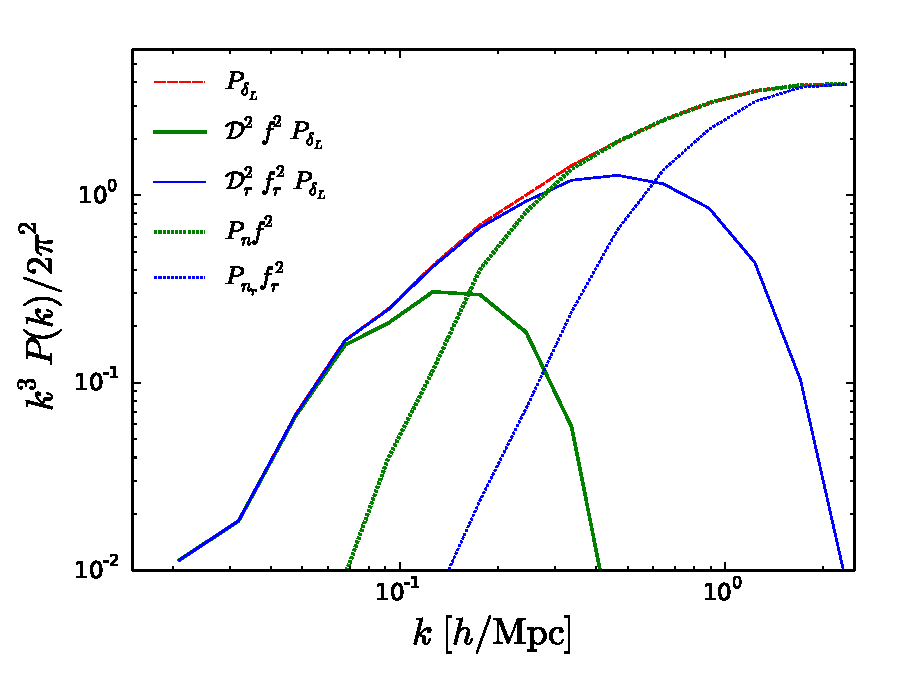
\includegraphics[width=0.48\textwidth]{fb.eps}
\end{center}
\vspace{-0.7cm}
\caption{The power spectra of the nonlinear and reconstructed density fields.}
\label{fig:ps}
\end{figure}

Figure \ref{fig:xcc} shows the cross-correlation coefficients of the nonlinear
and reconstruct density field with the linear density field.

\begin{figure}[tbp]
\begin{center}
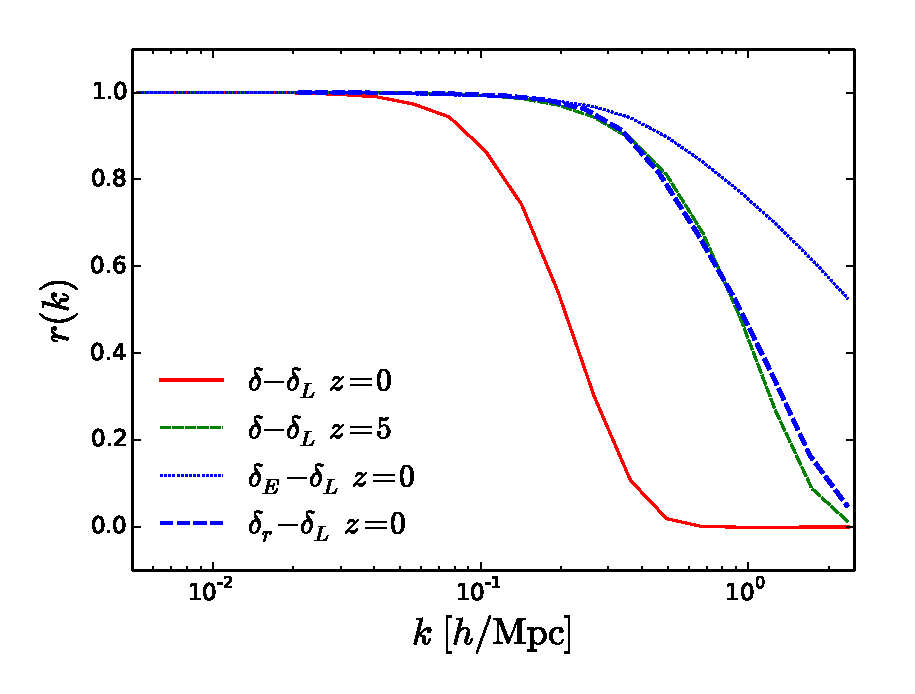
\includegraphics[width=0.48\textwidth]{fa.eps}
\end{center}
\vspace{-0.7cm}
\caption{The cross-correlation coefficients of the nonlinear and reconstructed 
density fields with the linear density field.}
\label{fig:xcc}
\end{figure}

Figure shows the PDFs of the density fields and displacement fields.

\begin{figure}[tbp]
\begin{center}
\includegraphics[width=0.48\textwidth]{pdf-1.eps}
\end{center}
\vspace{-0.7cm}
\caption{The PDFs of the reconstructed and linear density fields.}
\label{fig:pdf}
\end{figure}


%\begin{figure}[tbp]
%\begin{center}
%\includegraphics[width=0.48\textwidth]{map0256-064.eps}
%\end{center}
%\vspace{-0.7cm}
%\caption{The density field and the deformed grids. The length is 
%$300 \mr{Mpc}/h$.}
%\label{fig:map1}
%\end{figure}

{\it Discussions.}---
The reconstructed nonlinear displacement can be further ...
before apply to real data, consider RSD, halo fields, SDSS main samples ...
Peculiar velocity cosmology, predicting the displacement, robust measurement of
vlomue weighted velocity field, free of sampling artifact, and good at 
predicting the velocity field from the density field. also important for the
kSZ reconstruction

neutrino mass measurement, nonlinearity is fully exploitted. also important for
the velocity field reconstruction for measuring the dipole

%=======================================

The simulations were performed on the BGQ supercomputer at the SciNet HPC 
Consortium. SciNet is funded by the Canada Foundation for Innovation under 
the auspices of Compute Canada, the Government of Ontario, the Ontario Research 
Fund Research Excellence, and the University of Toronto.
We acknowledge the support of the Chinese MoST 863 program under Grant 
No. 2012AA121701, the CAS Science Strategic Priority Research Program 
XDB09000000, the NSFC under Grant No. 11373030, IAS at Tsinghua University, 
 and NSERC.
The Dunlap Institute is funded through an endowment established by the David Dunlap family and the University of Toronto.
Research at the Perimeter Institute is supported by the Government of Canada
through Industry Canada and by the Province of Ontario through the Ministry of
Research $\&$ Innovation.

\bibliographystyle{apsrev}
\bibliography{3d}

\end{document}
